\chapter{Observing the Cold Interstellar Medium}
\label{ch:obscold}

\marginnote{\textbf{Suggested background reading:}
\begin{itemize}
\item \href{http://adsabs.harvard.edu/abs/2012ARA\%26A..50..531K}{Kennicutt, R.~C., \& Evans, N.~J. 2012, ARA\&A, 50, 531}, sections $1-2$ \nocite{kennicutt12a}
\end{itemize}
}

This first chapter focuses on observations of interstellar gas. Because the interstellar clouds that form stars are generally cold, most (but not all) of these techniques require in infrared, sub-millimeter, and radio observations. Interpretation of the results is often highly non-trivial. This will naturally lead us to review some of the important radiative transfer physics that we need to keep in mind to understand the observations. With this background complete, we will then discuss the phenomenology of interstellar gas derived from these observations.

\section{Observing Techniques}

\subsection{The Problem of H$_2$}

\begin{marginfigure}
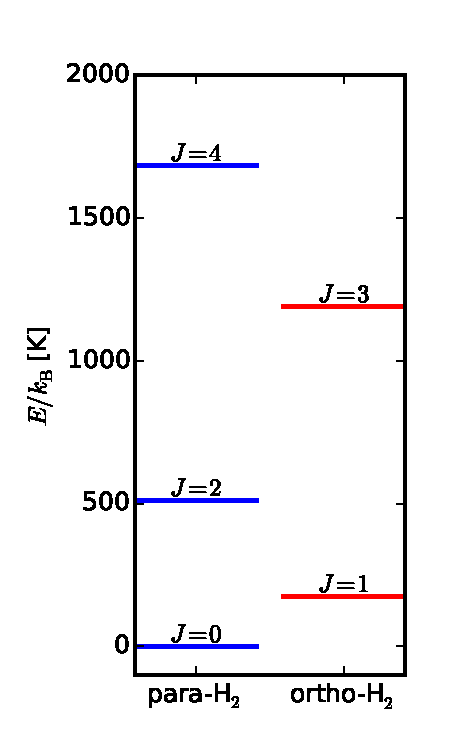
\includegraphics[width=\linewidth]{h2levels}
\caption[H$_2$ level diagram]{
\label{fig:h2levels}
Level diagram for the rotational levels of para- and ortho-H$_2$, showing the energy of each level. Level data are taken from \url{http://www.gemini.edu/sciops/instruments/nir/wavecal/h2lines.dat}.
}
\end{marginfigure}

Before we dive into all the tricks we use to observe the dense interstellar medium (ISM), we have to start at the question of why it is necessary to be so clever. Hydrogen is the most abundant element, and when it is in the form of free atomic hydrogen, it is relatively easy to observe. Hydrogen atoms emit radio waves at a wavelength of 21 cm (1.4 GHz), associated with a hyperfine transition from a state in which the spin of the electron is parallel to that of the proton to a state where it is anti-parallel. The energy difference between these two states corresponds to a temperature $\ll 1$ K, so even in cold regions it can be excited. This line is seen in the Milky Way and in many nearby galaxies.
  
However, at the high densities where stars form, hydrogen tends to be molecular rather than atomic, and H$_2$ is extremely hard to observe directly. To understand why, we can look at an energy level diagram for rotational levels of H$_2$ (Figure \ref{fig:h2levels}). A diatomic molecule like H$_2$ has three types of excitation: electronic (corresponding to excitations of one or more of the electrons), vibrational (corresponding to vibrational motion of the two nuclei), and rotational (corresponding to rotation of the two nuclei about the center of mass). Generally electronic excitations are highest in energy scale, vibrational are next, and rotational are the lowest in energy. Thus the levels shown in Figure \ref{fig:h2levels} are the ones that lie closest to ground.

For H$_2$, the first thing to notice is that the first excited state, the $J=1$ rotational state, is $175$ K above the ground state. Since the dense ISM where molecules form is often also cold, $T\sim 10$ K (as we will see later), almost no molecules will be in this excited state. However, it gets even worse: H$_2$ is a homonuclear molecule, and for reasons of symmetry $\Delta J = 1$ radiative transitions are forbidden in homonuclear molecules. Indeed, there is no electronic process by which a hydrogen molecule with odd $J$ to turn into one with even $J$, and vice versa, because the allowed parity of $J$ is determined by the spins of the hydrogen nuclei. We refer to the even $J$ state as para-H$_2$, and the odd $J$ state as ortho-H$_2$.

The observational significance of this is that there is no $J=1\rightarrow 0$ emission. Instead, the lowest-lying transition is the $J=2\rightarrow 0$ quadrupole. This is very weak, because it's a quadrupole. More importantly, however, the $J=2$ state is 510 K above the ground state. This means that, for a population in equilibrium at a temperature of 10 K, the fraction of molecules in the $J=2$ state is $\sim e^{-510/10} \approx 10^{-22}$!\footnote{This oversimplifies things quite a bit, because in real molecular clouds there are usually shocked regions where the temperature is much greater than 10 K, and H$_2$ rotational emission is routinely observed from them. However, this emission tracers rare gas that is much hotter than the mean temperature in a cloud, not the bulk of the mass, which is cold.} In effect, in a molecular cloud there are simply no H$_2$ molecules in states capable of emitting. The reason such a high temperature is required to excite the H$_2$ molecule is its low mass: for a quantum oscillator or rotor, the level spacing varies with reduced mass as $m^{-1/2}$. Thus the levels of H$_2$ are much farther apart than the levels of other diatomic molecules (e.g., CO, O$_2$, N$_2$). It is the low mass of the hydrogen atom that creates our problems.
  
Given this result, we see that, for the most part, observations of the most abundant species can only be done by proxy. Only in very rare circumstances is it possible to observe H$_2$ directly -- usually when there is a bright background UV source that allows us to see it in UV absorption rather than in emission. Since these circumstances do not generally prevail, we are forced to consider alternatives.

\subsection{Dust Emission}

The most conceptually straightforward proxy technique we use to study star-forming clouds is thermal dust emission. Interstellar gas clouds are always mixed with dust, and the dust grains emit thermal radiation that we can observe. The gas, in contrast, does not emit thermal radiation because it is nowhere near dense enough to reach equilibrium with the radiation field. Instead, gas emission comes primarily in the form of lines, which we will discuss below.
  
Consider a cloud of gas of mass density $\rho$ mixed with dust grains at a temperature $T$. The gas-dust mixture has an absorption opacity $\kappa_{\nu}$ to radiation at frequency $\nu$. Although the vast majority of the mass is in gas rather than dust, the opacity will be almost entirely due to the dust grains except for frequencies that happen to match the resonant absorption frequencies of atoms and molecules in the gas. Here we follow the standard astronomy convention that $\kappa_{\nu}$ is the opacity per gram of material, with units of cm$^2$ g$^{-1}$, i.e., we assign the gas an effective cross-sectional area that is blocked per gram of gas. For submillimeter observations, typical values of $\kappa_{\nu}$ are $\sim 0.01$ cm$^{2}$ g$^{-1}$. Figure \ref{fig:draine03opacity} shows a typical extinction curve for Milky Way dust.

\begin{marginfigure}
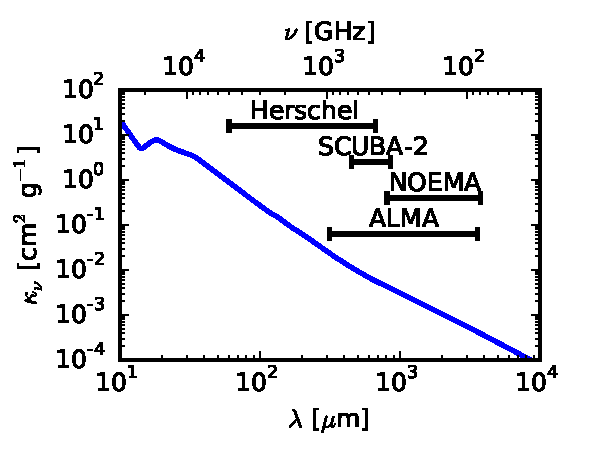
\includegraphics[width=\linewidth]{draine03opacity}
\caption[Dust absorption opacity]{
\label{fig:draine03opacity}
Milky Way dust absorption opacities per unit gas mass as a function of wavelength $\lambda$ and frequency $\nu$ in the infrared and sub-mm range, together with wavelength coverage of selected observational facilities. Dust opacities are taken from the model of \citet{draine03a} for $R_V = 5.5$.
}
\end{marginfigure}

Since essentially no interstellar cloud has a surface density $> 100$ g cm$^{-2}$, absorption of radiation from the back of the cloud by gas in front of it is completely negligible. Thus, we can compute the emitted intensity very easily. The emissivity for gas of opacity $\kappa_{\nu}$ is $j_{\nu} = \kappa_{\nu} \rho B_{\nu}(T)$, where $j_{\nu}$ has units of erg s$^{-1}$ cm$^{-3}$ sr$^{-1}$ Hz$^{-1}$, i.e.\ it describes (in cgs units) the number of ergs emitted in 1 second by 1 cm$^3$ of gas into a solid angle of 1 sr in a frequency range of 1 Hz. The quantity
\begin{equation}
B_{\nu}(T) = \frac{2 h\nu^3}{c^2} \frac{1}{e^{h\nu/\kb T}-1}
\end{equation}
is the Planck function.
  
Since none of this radiation is absorbed, we can compute the intensity transmitted along a given ray just by integrating the emission: 
  \begin{equation}
  I_{\nu} = \int j_{\nu} ds = \Sigma \kappa_{\nu} B_{\nu}(T) = \tau_{\nu} B_{\nu}(T)
  \end{equation}
where $\Sigma=\int \rho ds$ is the surface density of the cloud and $\tau_{\nu} = \Sigma \kappa_{\nu}$ is the optical depth of the cloud at frequency $\nu$. Thus if we observe the intensity of emission from dust grains in a cloud, we determine the product of the optical depth and the Planck function, which is determined solely by the observing frequency and the gas temperature. If we know the temperature and the properties of the dust grains, we can therefore determine the column density of the gas in the cloud in each telescope beam.

\begin{figure}
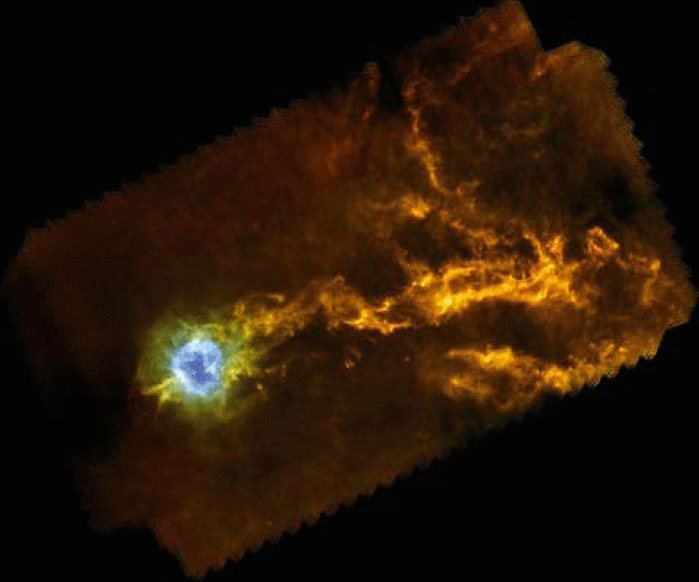
\includegraphics[width=\linewidth]{herschel_ic5146}
\caption[\textit{Herschel} map of IC 5146]{
\label{fig:herschel_ic5146}
Three-color composite image of IC 5146 taken by the SPIRE and PACS instruments aboard \textit{Herschel}. Red is SPIRE 500 $\mu$m, green is SPIRE 250 $\mu$m plus PACS 160 $\mu$m, and blue is PACS 70 $\mu$m. Credit: \citeauthor{arzoumanian11a}, A\&A, 529, L6, 2011, reproduced with permission \copyright\,ESO.
}
\end{figure}

Figure \ref{fig:herschel_ic5146} show an example result using this technique. The advantage of this approach is that it is very straightforward. The major uncertainties are in the dust opacity, which we probably don't know better than a factor of few level, and in the gas temperature, which is also usually uncertain at the factor of $\sim 2$ level. This produces a corresponding uncertainty in the conversion between dust emission and gas column density. Both of these can be improved substantially by observations that cover a wide variety of wavelengths, since these allow one to simultaneously fit the column density, dust opacity curve, and dust temperature.

Before the \textit{Herschel} satellite (launched in 2009) such multi-wavelength observations were rare, because most of the dust emission was in at far-infrared wavelengths of several hundred $\mu$m that are inaccessible from the ground. \textit{Herschel} was specifically targeted at this wavelength range, and has greatly improved our knowledge of cloud properties from dust emission.

\subsection{Dust Absorption}

A second related technique is, instead of looking at dust emission, looking at absorption of background starlight by dust, usually in the near infrared. In this case the calculation is even simpler. One measures the extinction of the background star and then simply divides by the gas opacity to get a column density. Probably the best example of this technique is the Pipe Nebula (Figure \ref{fig:pipe_lombardi06}).  

\begin{figure}
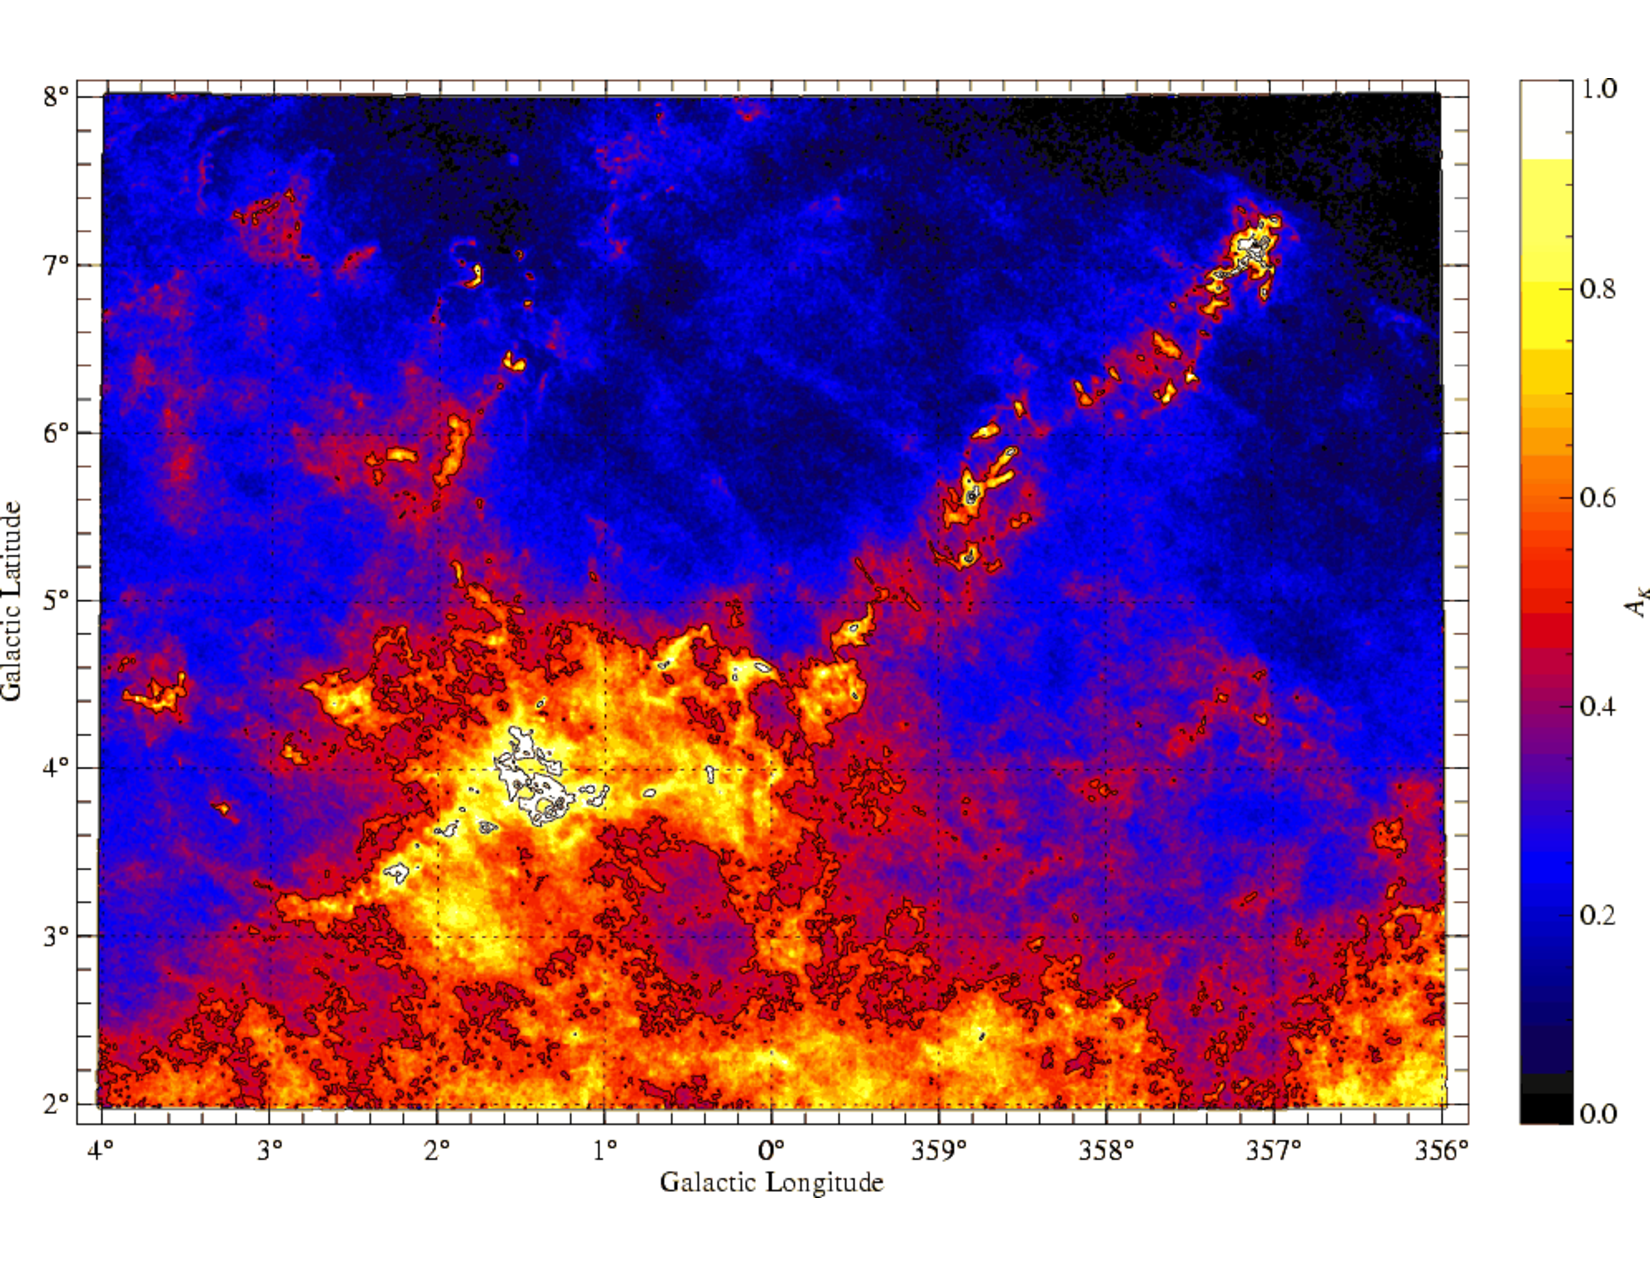
\includegraphics[width=\linewidth]{pipe_lombardi06}
\caption[Dust extinction map of the Pipe Nebula]{
\label{fig:pipe_lombardi06}
Extinction map of the Pipe Nebula. The color scale shows the extinction in K band. Credit: \citeauthor{lombardi06a}, A\&A, 454, 781, 2006, reproduced with permission \copyright\,ESO.
}
\end{figure}

The advantages of this compared to dust thermal emission are threefold. First, since stars are bright compared to interstellar dust grains, and the observations are done in the near IR rather than the sub-mm, the available resolution is much, much higher. Second, since opacity doesn't depend on temperature, the uncertainty in converting what we see into a column density is reduced. Third, we know the dust opacity curve in the near infrared considerably better than we know it in the far-IR or sub-mm, further reducing the uncertainty. However, there are also drawbacks to this method. Due to the comparatively higher opacity in the infrared, it is only possible to use this technique for fairly diffuse regions; in denser regions the background stars are completely extincted. Moreover, one needs a good, clean field of background stars to get something like a map, and only a few clouds have such favorable geometry.


\subsection{Molecular Lines}
\label{ssec:molecular_lines}

Much of what we know about star forming gas comes from observations of line emission. These are usually the most complex measurements in terms of the modeling and theory required to understand them. However, they are also by far the richest in terms of the information they provide. They are also among the most sensitive, since the lines can be very bright compared to continuum emission. Indeed, the great majority of what we know about the ISM beyond the local group comes from studying emission in the rotational lines of the CO molecule, because these (plus the C~\textsc{ii} line found in atomic regions) are by far the easiest types of emission to detect from the cold ISM.

The simplest line-emitting system is an atom or molecule with exactly two energy states, but this example contains most of the concepts we will need. The generalization of these results to a multi-level system is given in Appendix \ref{app:multilevel_atoms}.

\paragraph{Einstein Coefficients and Collision Rates}

Consider an atom or molecule of species $X$ with two non-degenerate states that are separated by an energy $E$. Suppose we have a gas of such particles with number density $n_X$ at temperature $T$. The number density of atoms in the ground state is $n_0$ and the number density in the excited state is $n_1$. At first suppose that this system does not radiate. In this case collisions between the atoms will eventually bring the two energy levels into thermal equilibrium, and it is straightforward to compute $n_0$ and $n_1$. They just follow a Maxwellian distribution, so $n_1/n_0 = e^{-E/k_B T}$, and thus we have $n_0 = n_X /Z$ and $n_1 = n_X e^{-E/k_B T}/Z$, where $Z=1+e^{-E/k_B T}$ is the partition function.

Now let us consider radiative transitions between these states. There are three processes: spontaneous emission, stimulated emission, and absorption, which are described by the three Einstein coefficients. In studying star formation, we can often ignore stimulated emission and absorption, because the ambient radiation field is so weak that these processes occur at negligible rates. The exception to this is when lines become optically thick, so there are a lot of line photons bouncing around trapped inside a structure, or when the frequency of the transition in question is at very low energy, and interactions with CMB photons become significant. However, for simplicity we will begin by just focusing on spontaneous emission and ignoring absorption and stimulated emission. The full statistical mechanics problem including these processes is discussed in Appendix \ref{app:multilevel_atoms}.

An atom in the excited state can spontaneously emit a photon and decay to the ground state. The rate at which this happens is described by the Einstein coefficient $A_{10}$, which has units of s$^{-1}$. Its meaning is simply that a population of $n_1$ atoms in the excited state will decay to the ground state by spontaneous emission at a rate 
\begin{equation}
\left(\frac{dn_1}{dt}\right)_{\rm spon.~emis.} = -A_{10} n_1.
\end{equation}
In cgs units this quantity is measured in atoms per cm$^3$ per s, and this expression is equivalent to saying that the $e$-folding time for decay is $1/A_{10}$ seconds. For most of the molecules we will be considering in this book, decay times are typically at most a few centuries, which is short compared to pretty much any time scale associated with star formation. Thus if spontaneous emission were the only process at work, all molecules would quickly decay to the ground state and we wouldn't see any emission.

However, in the dense interstellar environments where stars form, collisions occur frequently enough to create a population of excited molecules. Of course collisions involving excited molecules can also cause de-excitation, with the excess energy going into recoil rather than into a photon. Since hydrogen molecules are almost always the most abundant species in the dense regions we're going to think about, with helium second, we can generally only consider collisions between our two-level atom and those partners. For the purposes of this exercise, we'll take an even simpler approach and ignore everything but H$_2$. Putting He back into the picture is easy, as it just requires adding extra collision terms that are completely analogous to the ones we will write down.

The rate at which collisions cause transitions between states is a horrible quantum mechanical problem. We cannot even confidently calculate the energy levels of single isolated molecules except in the simplest cases, let alone the interactions between two colliding ones at arbitrary velocities and relative orientations. Exact calculations of collision rates are generally impossible. Instead, we either make due with approximations (at worst), or we try to make laboratory measurements. Things are bad enough that, for example, we often assume that the rates for collisions with H$_2$ molecules and He atoms are related by a constant factor.

Fortunately, as astronomers we generally leave these problems to chemists, and instead do what we always do: hide our ignorance behind a parameter. We let the rate at which collisions between species $X$ and H$_2$ molecules induce transitions from the ground state to the excited state be
\begin{equation}
\left(\frac{dn_1}{dt}\right)_{\rm coll.~exc.} = k_{01} n_0 n,
\end{equation}
where $n$ is the number density of H$_2$ molecules and $k_{01}$ has units of cm$^3$ s$^{-1}$. In general $k_{01}$ will be a function of the gas kinetic temperature $T$, but not of $n$ (unless $n$ is so high that three-body processes start to become important, which is almost never the case in the ISM). 

The corresponding rate coefficient for collisional de-excitation is $k_{10}$, and the collisional de-excitation rate is
\begin{equation}
\left(\frac{dn_1}{dt}\right)_{\rm coll.~de-exc.} = -k_{10} n_1 n.
\end{equation}
A little thought should suffice to convince the reader that $k_{01}$ and $k_{10}$ must have a specific relationship. Consider an extremely dense region where $n$ is so large that collisional excitation and de-excitation both occur much, much more often than spontaneous emission, and we can therefore neglect the spontaneous emission term in comparison to the collisional ones. If the gas is in equilibrium then we have
\begin{eqnarray}
\frac{dn_1}{dt} = \left(\frac{dn_1}{dt}\right)_{\rm coll.~exc.} + \left(\frac{dn_1}{dt}\right)_{\rm coll.~de-exc.} & = & 0 \\
n (k_{01} n_0 - k_{10} n_1) & = & 0.
\end{eqnarray}
However, we also know that the equilibrium distribution is a Maxwellian, so $n_1/n_0 = e^{-E/k_B T}$. Thus we have
\begin{eqnarray}
n n_0 (k_{01} - k_{10} e^{-E/k_B T}) & = & 0 \\
k_{01} & = & k_{10} e^{-E/k_B T}.
\label{eq:detailed_balance}
\end{eqnarray}
This argument applies equally well between a pair of levels even for a complicated molecule with many levels instead of just 2. Thus, we only need to know the rate of collisional excitation or de-excitation between any two levels to know the reverse rate.

\paragraph{Critical Density and Density Inference}

We are now in a position to write down the full equations of statistical equilibrium for the two-level system. In so doing, we will see that we can immediately use line emission to learn a great deal about the density of gas. In equilibrium we have
\begin{eqnarray}
\frac{dn_1}{dt} & = & 0 \\
n_1 A_{10} + n n_1 k_{10} -n n_0 k_{01} & = & 0 \\
\frac{n_1}{n_0} \left(A_{10} + k_{10}n\right) - k_{01} n & = & 0\\
\frac{n_1}{n_0} & = & \frac{k_{01} n}{A_{10}+k_{10} n}\\
& = & e^{-E/k_B T} \frac{1}{1+A_{10}/(k_{10} n)}
\end{eqnarray}
This physical meaning of this expression is clear. If radiation is negligible compared to collisions, i.e., $A_{10} \ll k_{10} n$, then the ratio of level populations approaches the Maxwellian ratio $e^{-E/k_B T}$. As radiation becomes more important, i.e., $A_{10}/(k_{10} n)$ get larger, the fraction in the upper level drops -- the level population is sub-thermal. This is because radiative decays remove molecules from the upper state faster than collisions re-populate it.

Since the collision rate depends on density and the radiative decay rate does not, the balance between these two processes depends on density. This make it convenient to introduce a critical density $n_{\rm crit}$, defined by
\begin{equation}
\label{eq:ncrit}
n_{\rm crit} = \frac{A_{10}}{k_{10}},
\end{equation}
so that
\begin{equation}
\frac{n_1}{n_0} = e^{-E/k_B T} \frac{1}{1+n_{\rm crit}/n}.
\end{equation}
At densities much larger than $n_{\rm crit}$, we expect the level population to be close to the Maxwellian value, and at densities much smaller than $n_{\rm crit}$ we expect the upper state to be under-populated relative to Maxwellian; $n_{\rm crit}$ itself is simply the density at which radiative and collisional de-excitations out of the upper state occur at the same rate.

This process of thermalization has important consequences for the line emission we see from molecules. The energy emission rate per molecule from the line is 
\begin{eqnarray}
\frac{\mathcal{L}}{n_X} & = & \frac{E A_{10} n_1}{n_X} \\
& = & E A_{10} \frac{n_1}{n_0+n_1} \\
& = & E A_{10} \frac{n_1/n_0}{1+n_1/n_0} \\
& = & E A_{10} \frac{e^{-E/k_B T}}{1+e^{-E/k_B T}+n_{\rm crit}/n} \\
& = & E A_{10} \frac{e^{-E/k_B T}}{Z+n_{\rm crit}/n}
\end{eqnarray}
where again $Z$ is the partition function.

It is instructive to think about how this behaves in the limiting cases $n \ll n_{\rm crit}$ and $n\gg n_{\rm crit}$. In the limit $n\gg n_{\rm crit}$, the partition function $Z$ dominates the denominator, and we get $\mathcal{L}/n_X = E A_{10} e^{-E/k_B T}/Z$. This is just the energy per spontaneous emission, $E$, times the spontaneous emission rate, $A_{10}$, times the fraction of the population in the upper state when the gas is in statistical equilibrium, $e^{-E/k_B T}/Z$. This is density-independent, so this means that at high density the gas produces a fixed amount of emission per molecule of the emitting species. The total luminosity is just proportional to the number of emitting molecules.

For $n \ll n_{\rm crit}$, the second term dominates the denominator, and we get
\begin{equation}
\label{eq:cool_lowden}
\frac{\mathcal{L}}{n_X} \approx E A_{10} e^{-E/k_B T} \frac{n}{n_{\rm crit}}.
\end{equation}
Thus at low density each molecule contributes an amount of light that is proportional to the ratio of density to critical density. Note that this is the ratio of collision partners, i.e., of H$_2$, rather than the density of emitting molecules. The total luminosity varies as this ratio times the number of emitting molecules.

The practical effect of this is that different molecules tell us about different densities of gas in galaxies. Molecules with low critical densities reach the linear regime at low density, and since most of the mass tends to be at lower density, they probe this widespread, low-density component. Molecules with higher critical densities will have more of their emission contributed by higher density gas, and thus tell us about rarer, higher-density regions. This is all somewhat qualitative, since a transition between $\mathcal{L}/n_X \propto n$ and $\mathcal{L}/n_X \sim\mbox{constant}$ doesn't represent a particularly sharp change in behavior. Nonetheless, the luminosity ratios of lines with different critical densities are a very important diagnostic of the overall density distribution in the ISM.

As a caution, we should note that this is computed for optically thin emission. If the line is optically thick, we can no longer ignore stimulated emission and absorption processes, and not all emitted photons will escape from the cloud. In this case the effective critical density is reduced by a factor of the optical depth. CO, the most-commonly used tracer molecule, is usually optically thick.

\paragraph{Velocity and Temperature Inference}

We can also use molecular lines to infer the velocity and temperature structure of gas if the line in question is optically thin. For an optically thin line, the width of the line is determined primarily by the velocity distribution of the emitting molecules. The physics here is extremely simple. Suppose we have gas along our line of sight with a velocity distribution $\psi(v)$, i.e., the fraction of gas with velocities between $v$ and $v+dv$ is $\psi(v) dv$, and $\int_{-\infty}^{\infty} \psi(v) \, dv = 1$.

For an optically thin line, in the limit where natural and pressure-broadening of lines is negligible, which is almost always the case when observing the cold, dense, ISM, we can think of emission producing a delta function in frequency in the rest frame of the gas. There is a one-to-one mapping between velocity and frequency. Thus emission from gas moving at a velocity $v$ relative to us along our line of sight produces emission at a frequency $\nu \approx \nu_0 (1 - v/c)$, where $\nu_0$ is the central frequency of the line in the molecule's rest frame, and we assume $v/c \ll 1$. In this case the line profile is described trivially by $\phi(\nu)=\psi(c(1-\nu/\nu_0))$. 

We can measure $\phi(\nu)$ directly, and this immediately tells us the velocity distribution $\psi(v)$. In general the velocity distribution of the gas $\psi(v)$ is produced by a combination of thermal and non-thermal motions. Thermal motions arise from the Maxwellian velocity distribution of the gas, and produce a Maxwellian profile $\phi(\nu)\propto e^{-(\nu-\nu_{\rm cen})^2/2\sigma_\nu^2}$. Here $\nu_{\rm cen}$ is the central frequency of the line, which is $\nu_{\rm cen} = \nu_0 (1 - \bar{v}/c)$, where $\bar{v}$ is the mean velocity of the gas along our line of sight. The width is $\sigma_\nu = \nu_0 c^{-1}\sqrt{k_B T/\mu m_{\rm H}}$, where $T$ is the gas temperature and $\mu$ is the mean mass of the emitting molecule in units of hydrogen masses. This is just the 1D Maxwellian distribution.

Non-thermal motions involve bulk flows of the gas, and can produce a variety of velocity distributions depending how the cloud is moving. Unfortunately even complicated motions often produce distributions that look something like Maxwellian distributions, just because of the central limit theorem: if you throw together a lot of random junk, the result is usually a Gaussian / Maxwellian distribution. Figure \ref{fig:complete_ridge06} shows an example of velocity distributions measured in two nearby star-forming clouds.

\begin{marginfigure}
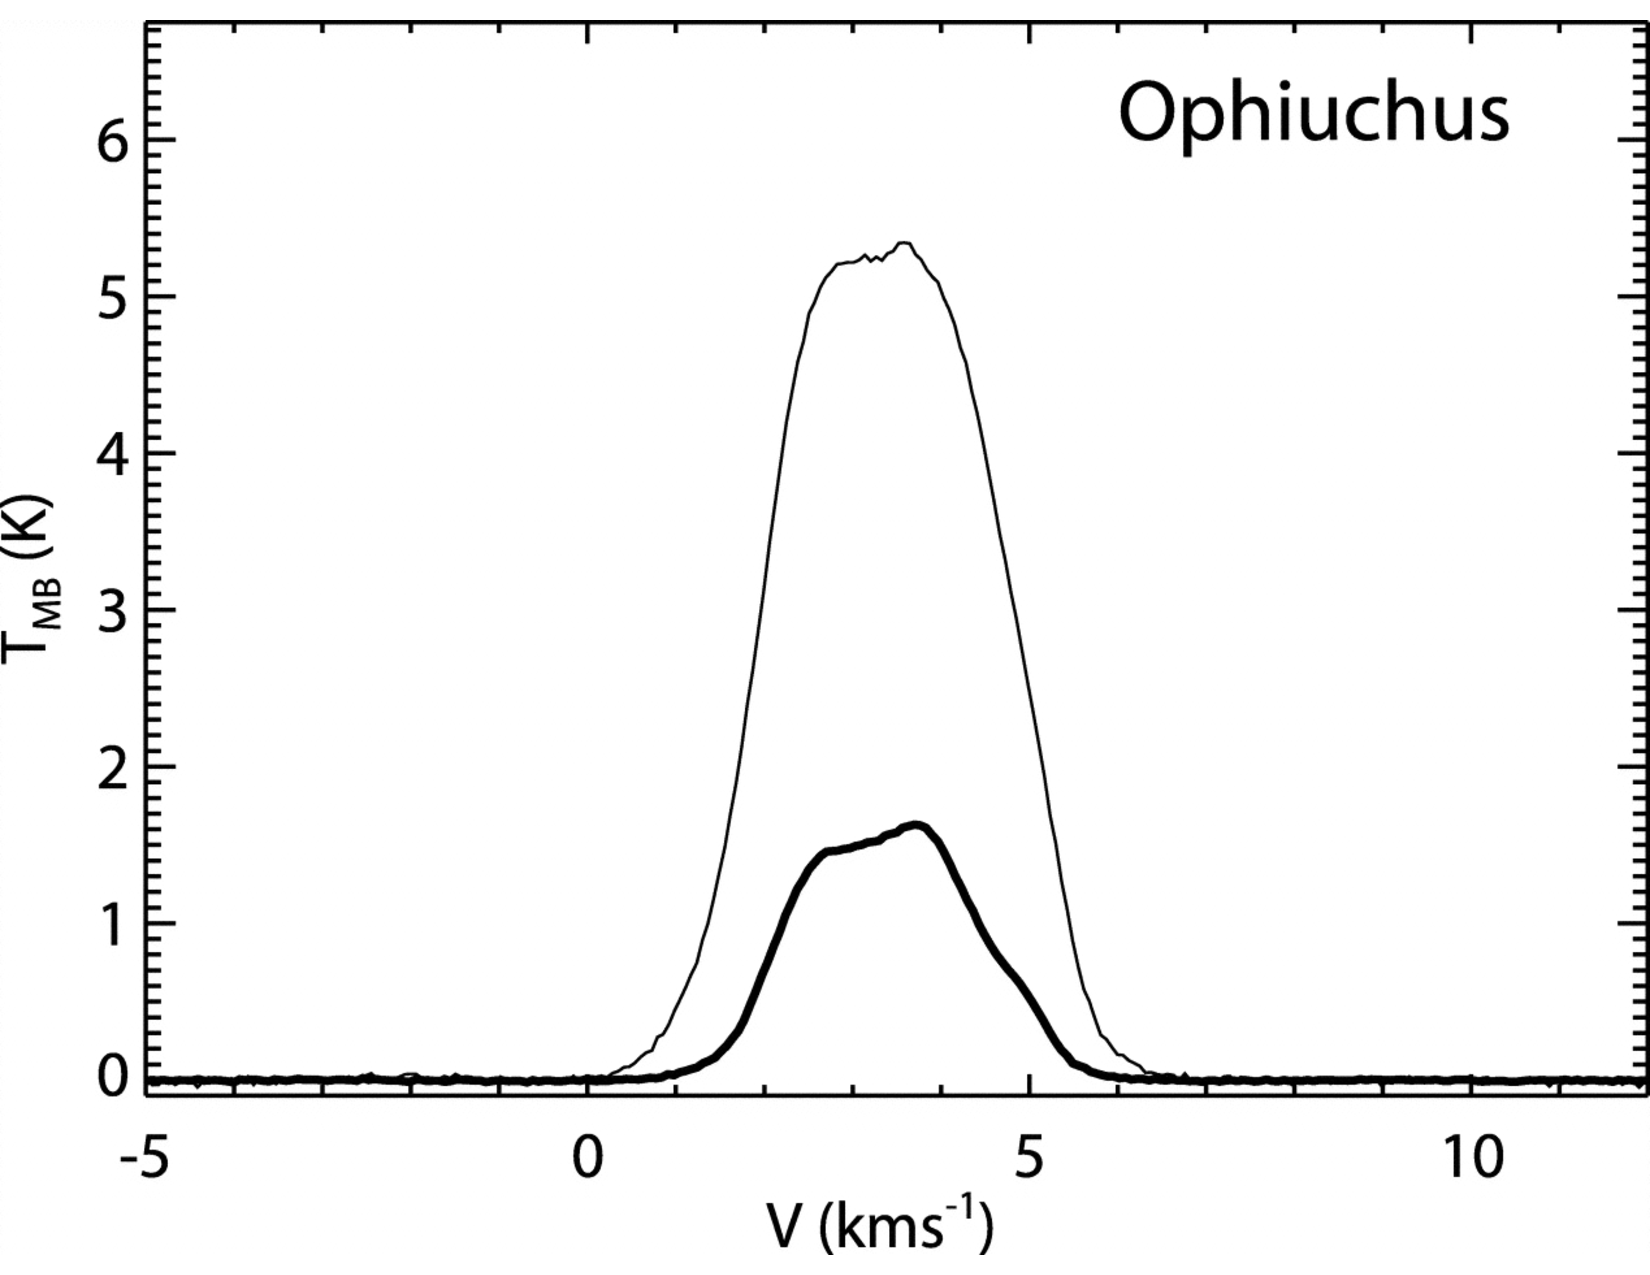
\includegraphics[width=\linewidth]{complete_ridge06a}
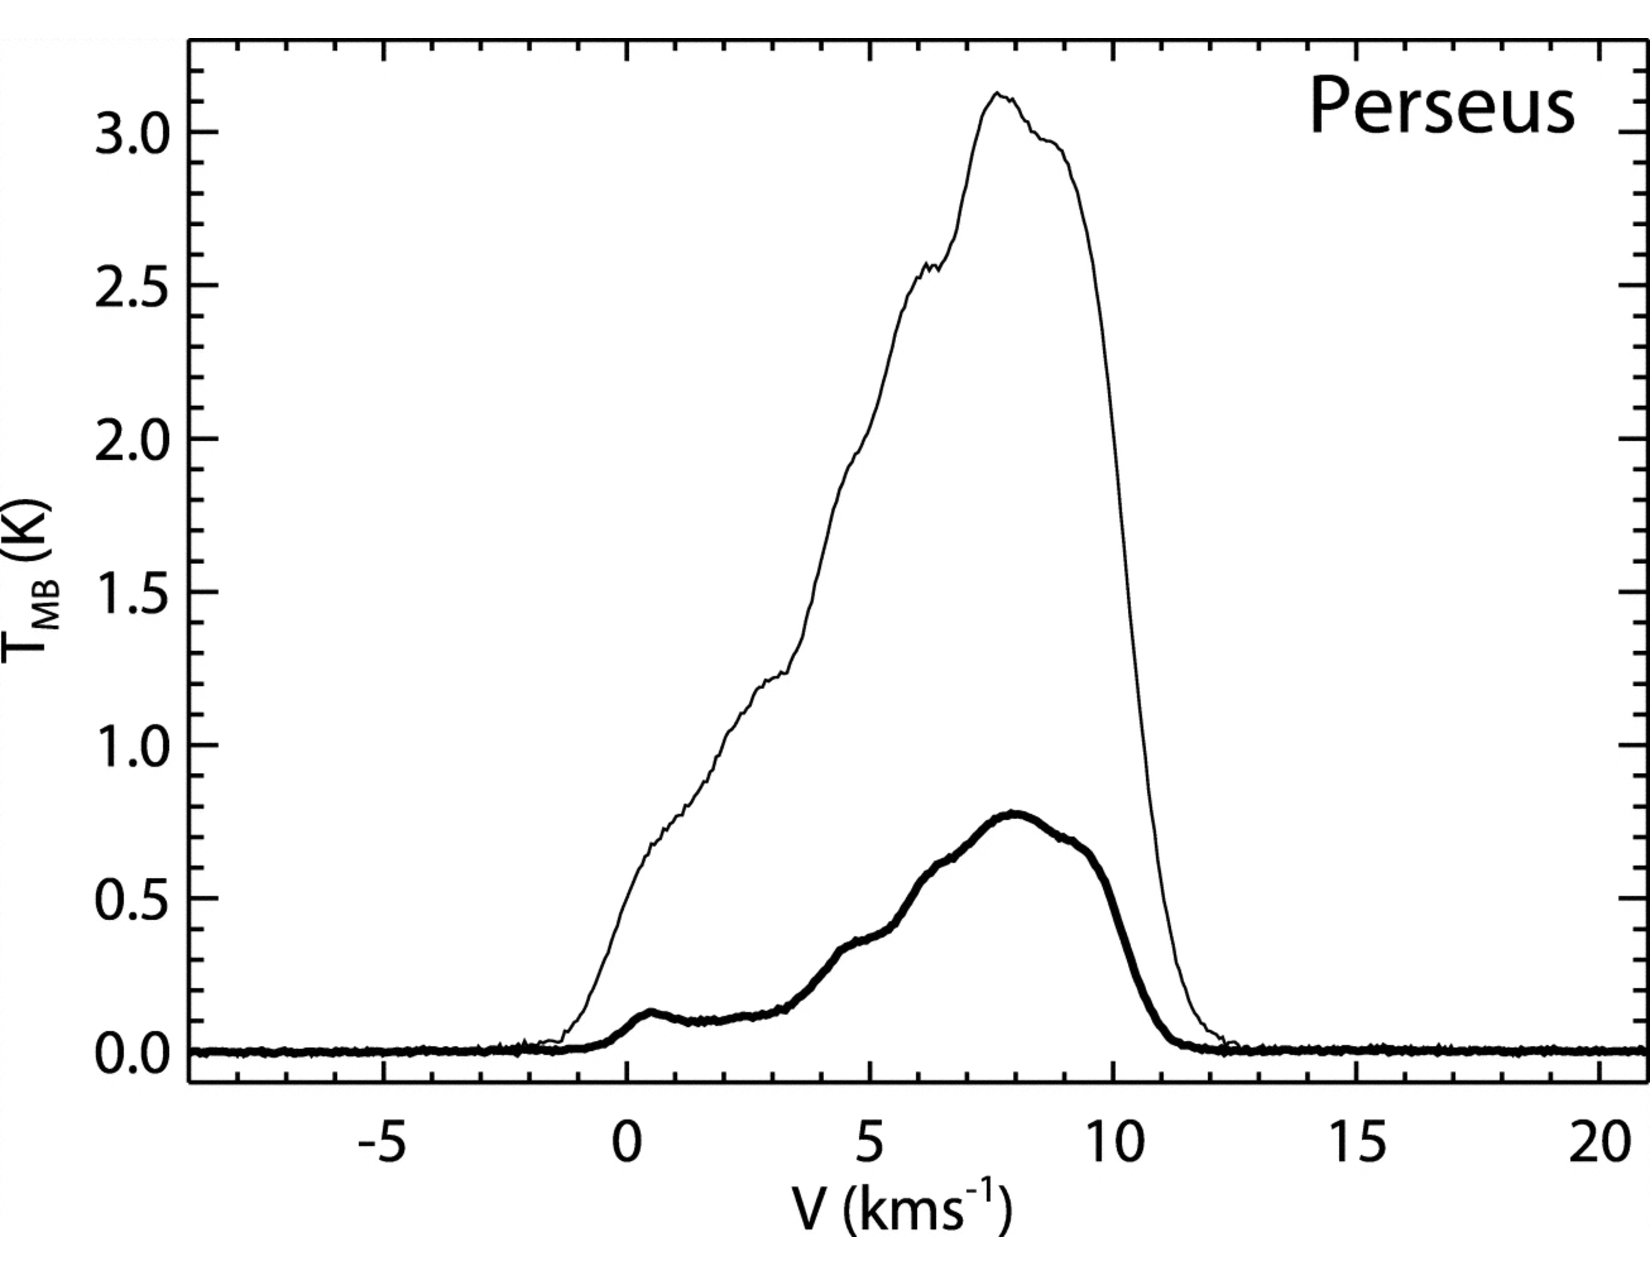
\includegraphics[width=\linewidth]{complete_ridge06b}
\caption[COMPLETE spectra of Ophiuchus and Perseus]{
\label{fig:complete_ridge06}
Position-integrated velocity distributions of $^{12}$CO (\textit{thin lines}) and $^{13}$CO (\textit{thick lines}) for the Ophiuchus and Perseus clouds, measured the COMPLETE survey. The $y$ axis shows the beam temperature. Credit: \citet{ridge06a}, \copyright\, AAS. Reproduced with permission.
}
\end{marginfigure}

Determining whether a given line profile reflects predominantly thermal or non-thermal motion requires that we have a way of estimating the temperature independently. This can often be done by observing multiple lines of the same species. Our expression
\begin{equation}
\frac{\mathcal{L}}{n_X} = E A_{10} \frac{e^{-E/k_B T}}{Z + n_{\rm crit}/n}
\end{equation}
shows that the luminosity of a particular optically thin line is a function of the temperature $T$, the density $n$, and the number density of emitting molecules $n_X$. If we observe three transitions of the same molecule, then we have three equations in three unknowns and we can solve for $n$, $n_X$, and $T$ independently. Certain molecules, because of their level structures, make this technique particularly clean. The most famous example of this is ammonia, NH$_3$.

\paragraph{Complications}

Before moving on it is worth mentioning some complications that make it harder to interpret molecular line data. The first is optical depth: for many of the strongest lines and most abundant species, the line becomes optically thick. As a result observations in the line show only the surface a given cloud; emission from the back side of the cloud is absorbed by the front side. One can still obtain useful information from optically thick lines, but it requires a bit more thought. We will return to the topic of what we can learn from optically thick lines in Chapter \ref{ch:gmcs}.

The second complication is chemistry and abundances. The formation and destruction of molecules in the ISM is a complicated problem, and in general the abundance of any given species depends on the density, temperature, and radiation environment of the the gas. At the edges of clouds, certain molecules may not be present because they are dissociated by the interstellar UV field. At high densities and low temperatures, many species freeze out onto the surfaces of dust grains. This is true for example of CO. One often sees that peaks in density found in dust emission maps correspond to local minima of CO emission. This is because in the densest parts of clouds CO goes out of the gas phase and forms CO ice on the surfaces of dust grains.  Thus one must always be careful to investigate whether changes in molecular line emission are due to changes in gas bulk properties (e.g., density, temperature) or due to changes in the abundance of the emitting species.


\section{Observational Phenomenology}

\subsection{Giant Molecular Clouds}

As discussed above, we usually cannot observe H$_2$ directly, so we are forced to do so by proxy. The most common proxy is the rotational lines of CO. These are useful because CO is the single most abundant molecule in the ISM after H$_2$, it tends to be found in the same places as H$_2$ (for reasons that will become clear in Chapter \ref{ch:microphysics}, and the CO molecule has a number of transitions that can be excited at the low temperatures found in molecular clouds -- for example the CO $J=1$ state is only 5.5 K above the ground state. Indeed, the CO molecule is the primary coolant of molecular gas, so its excitation in effect sets the molecular gas temperature. 

In Chapter \ref{ch:gmcs} we will discuss how one infers the mass of an observed gas cloud from CO emission, and for the moment we will take it for granted that one can do so. By mass the Milky Way's ISM inside the solar circle is roughly 70\% H~\textsc{i} and 30\% H$_2$. The molecular fraction rises sharply toward the galactic center, reaching near unity in the molecular ring at $\sim 3$ kpc, then falling to $\sim 10\%$ out where we are. In other nearby galaxies the proportions vary from nearly all H~\textsc{i} to nearly all H$_2$.

In galaxies that are predominantly H~\textsc{i}, like ours, the atomic gas tends to show a filamentary structure, with small clouds of molecular gas sitting on top of peaks in the H~\textsc{i} distribution. In galaxies with large-scale spiral structure, the molecular gas closely tracks the optical spiral arms. Figures \ref{fig:m33_imara} and \ref{fig:m51_schinnerer} show examples of the former and the latter, respectively. The physical reasons for the associations between molecular gas and H~\textsc{i}, and between molecular clouds and spiral arms, are an interesting point that we will discuss in Chapter \ref{ch:microphysics}. 

\begin{figure}
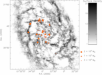
\includegraphics[width=\linewidth]{m33_imara}
\caption[Distribution of H~\textsc{i} and GMCs in M33]{
\label{fig:m33_imara}
Map of H~\textsc{i} in M33 (\textit{grayscale}), with giant molecular clouds detected in CO($1\rightarrow 0$) overlayed (\textit{circles}, sized by GMC mass). Credit: \citet{imara11b}, \copyright\, AAS. Reproduced with permission.
}
\end{figure}

\begin{figure}
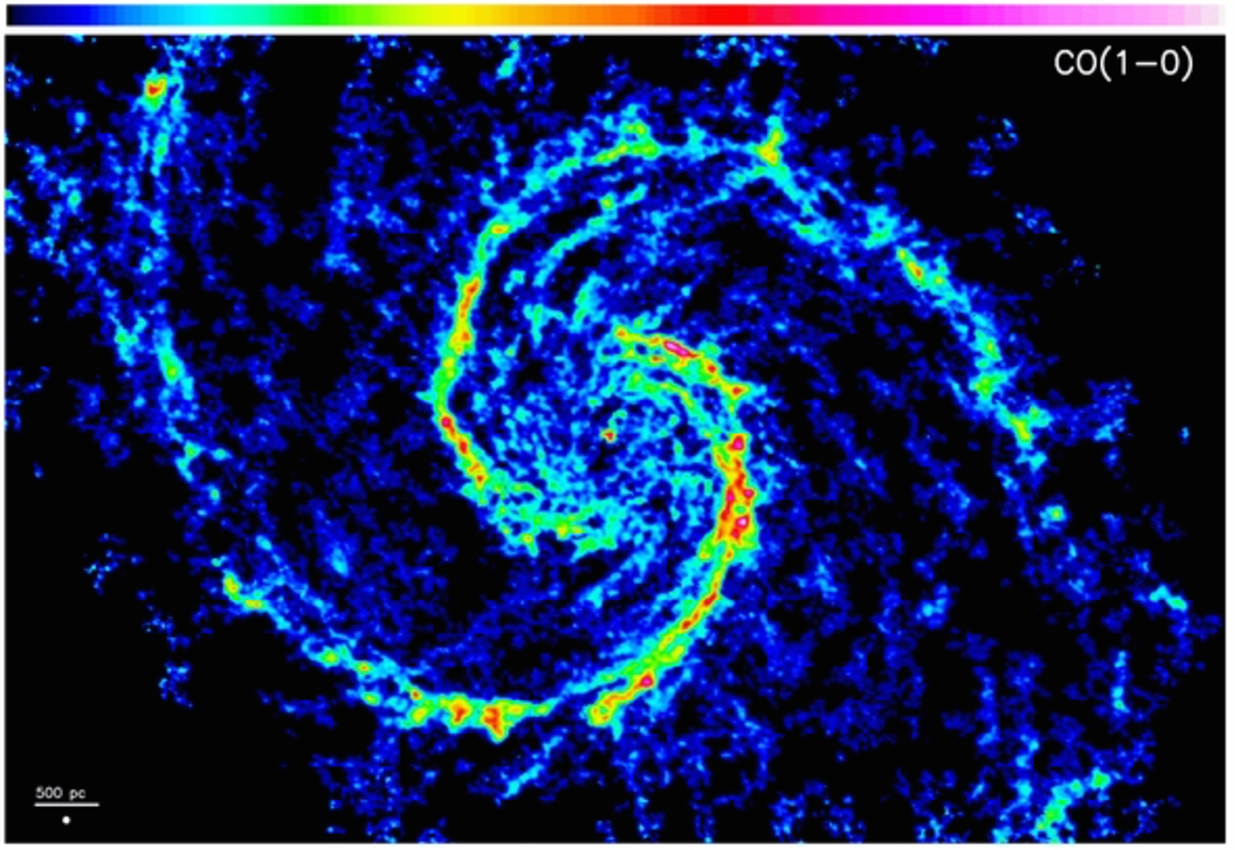
\includegraphics[width=\linewidth]{m51_schinnerer}
\caption[Distribution of CO($1\rightarrow 0$) emission in M51]{
\label{fig:m51_schinnerer}
Map of CO($1\rightarrow 0$) emission in M51, as measured by the PdBI Arcsecond Whirlpool Survey (PAWS) project. Credit: \citet{schinnerer13a}, \copyright\, AAS. Reproduced with permission.
}
\end{figure}

As the images show, molecular gas in galaxies that are predominantly atomic tends to be organized into discreet clouds, called giant molecular clouds (GMCs). These can have a range of masses; in the Milky Way the most massive are a few million $\msun$, but there is a spectrum that seems to continue down to at least $10^4$ $\msun$. This organization into GMCs is clearest where the gas is predominantly atomic. In regions where molecules make up most of the mass, the clouds begin to run together and it is no longer possible to identify discrete clouds in a meaningful way.

\subsection{Internal structure of GMCs}

Giant molecular clouds are not spheres. They have complex internal structures, as illustrated in Figure \ref{fig:perseus_sun06}. They tend to be highly filamentary and clumpy, with most of the mass in low density structures and only a little bit in very dense parts. However, if one computes a mean density by dividing the total mass by the rough volume occupied by the $^{12}$CO gas, the result is $\sim 100$ cm$^{-3}$. Typical size scales for GMCs are tens of pc -- the Perseus cloud shown in Figure \ref{fig:perseus_sun06} is a small one by Galactic standards, but the most massive ones are found predominantly in the molecular ring, so our high resolution images are all of nearby small ones.

\begin{figure}
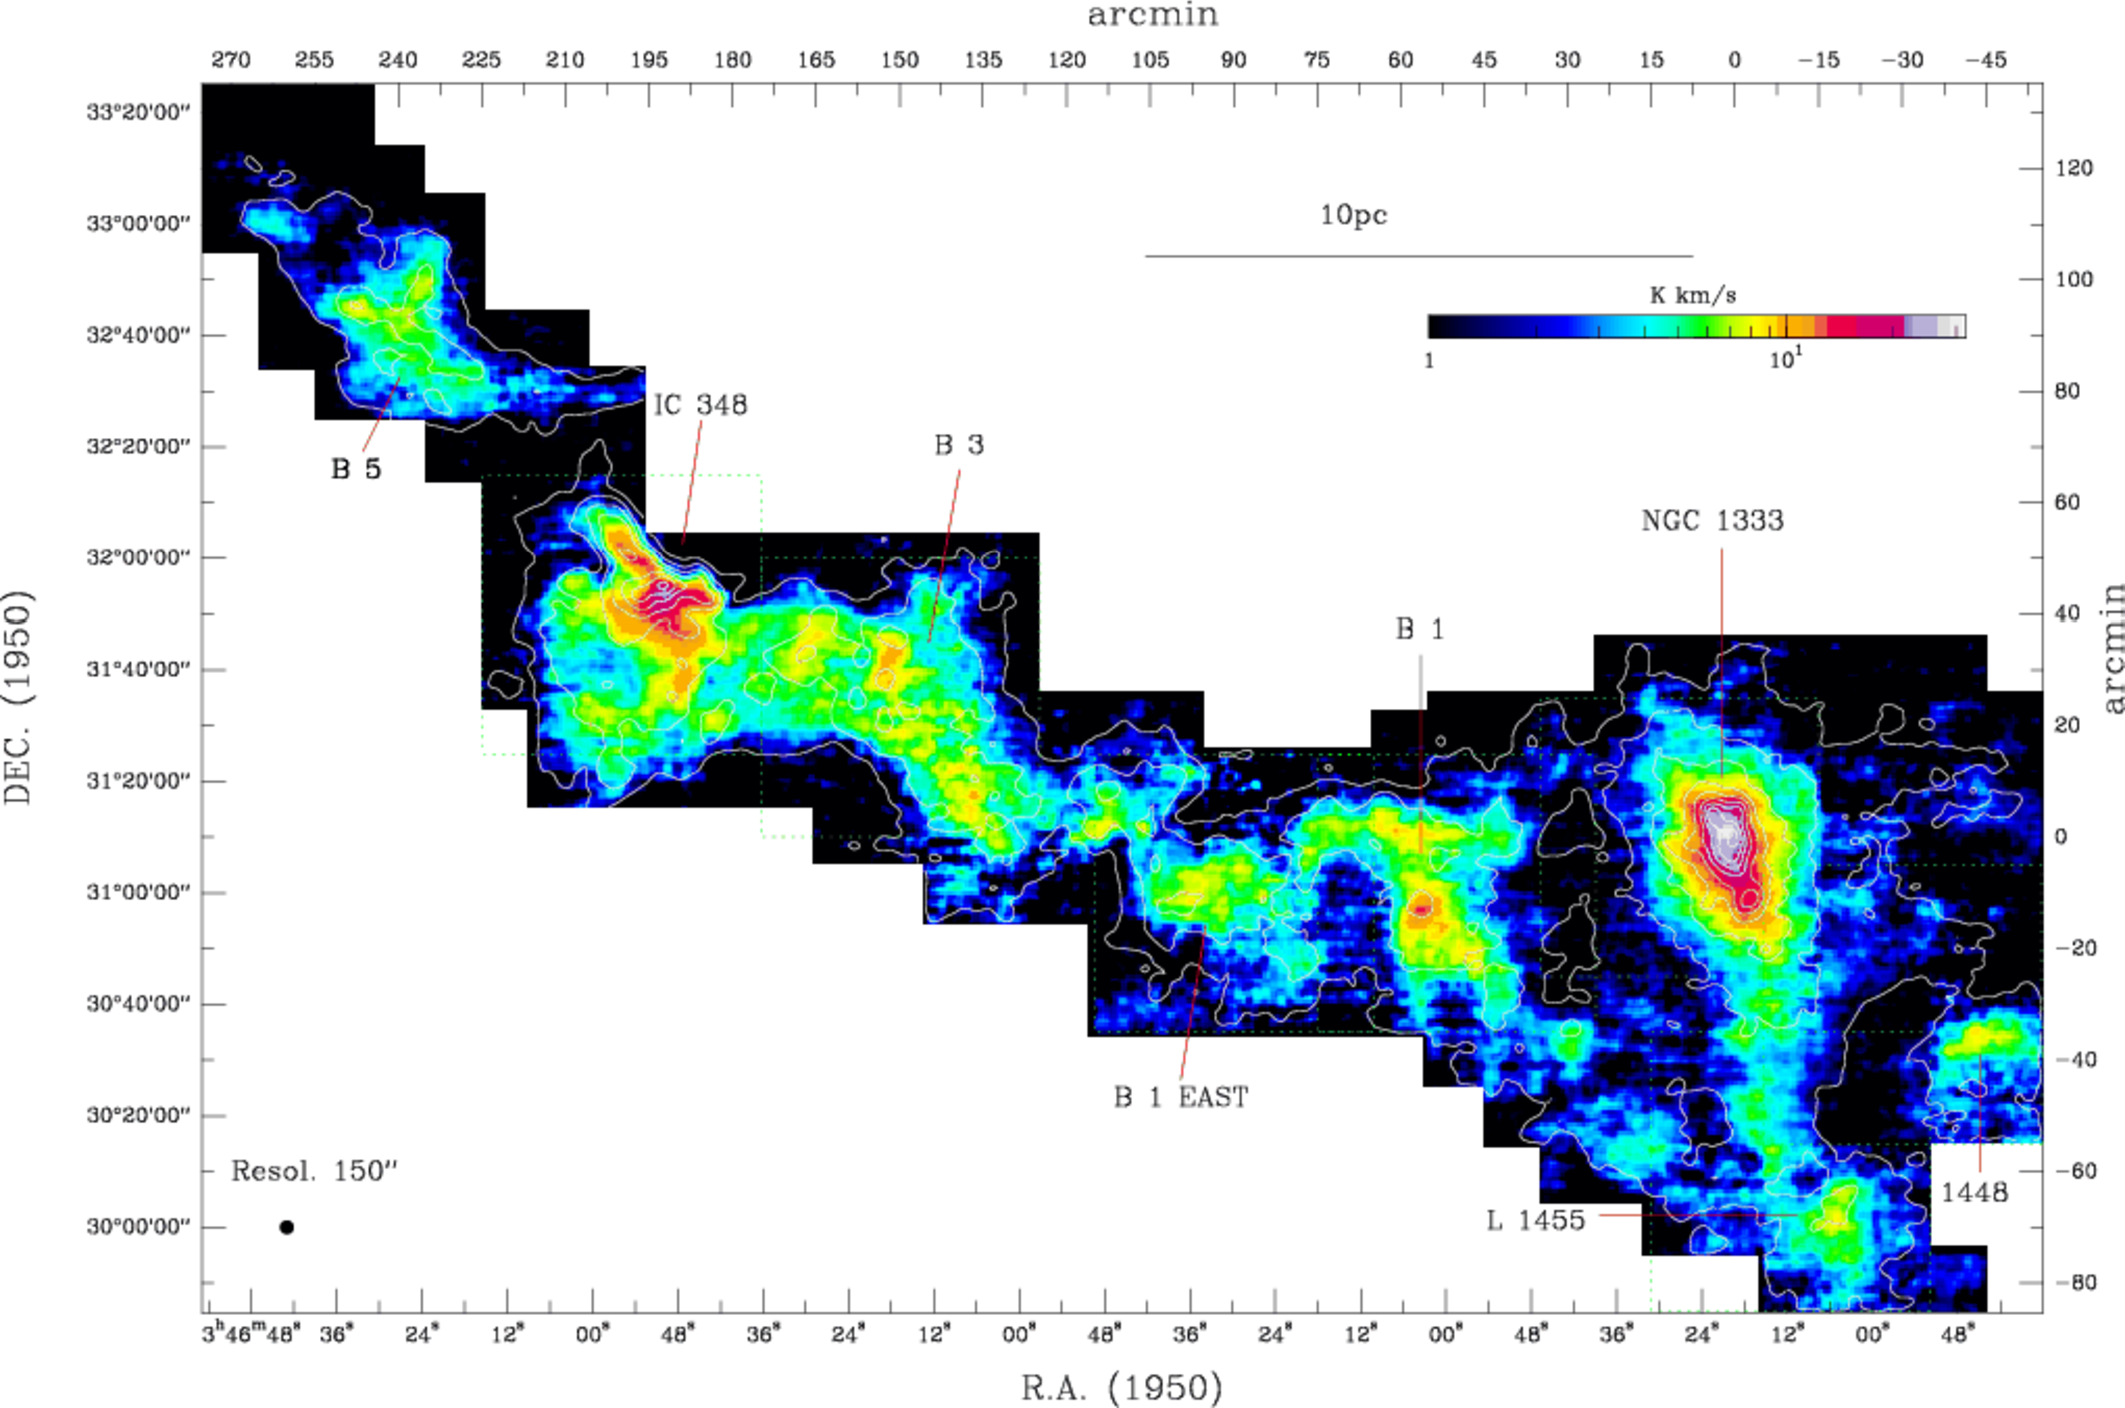
\includegraphics[width=\linewidth]{perseus_integrated_sun06}
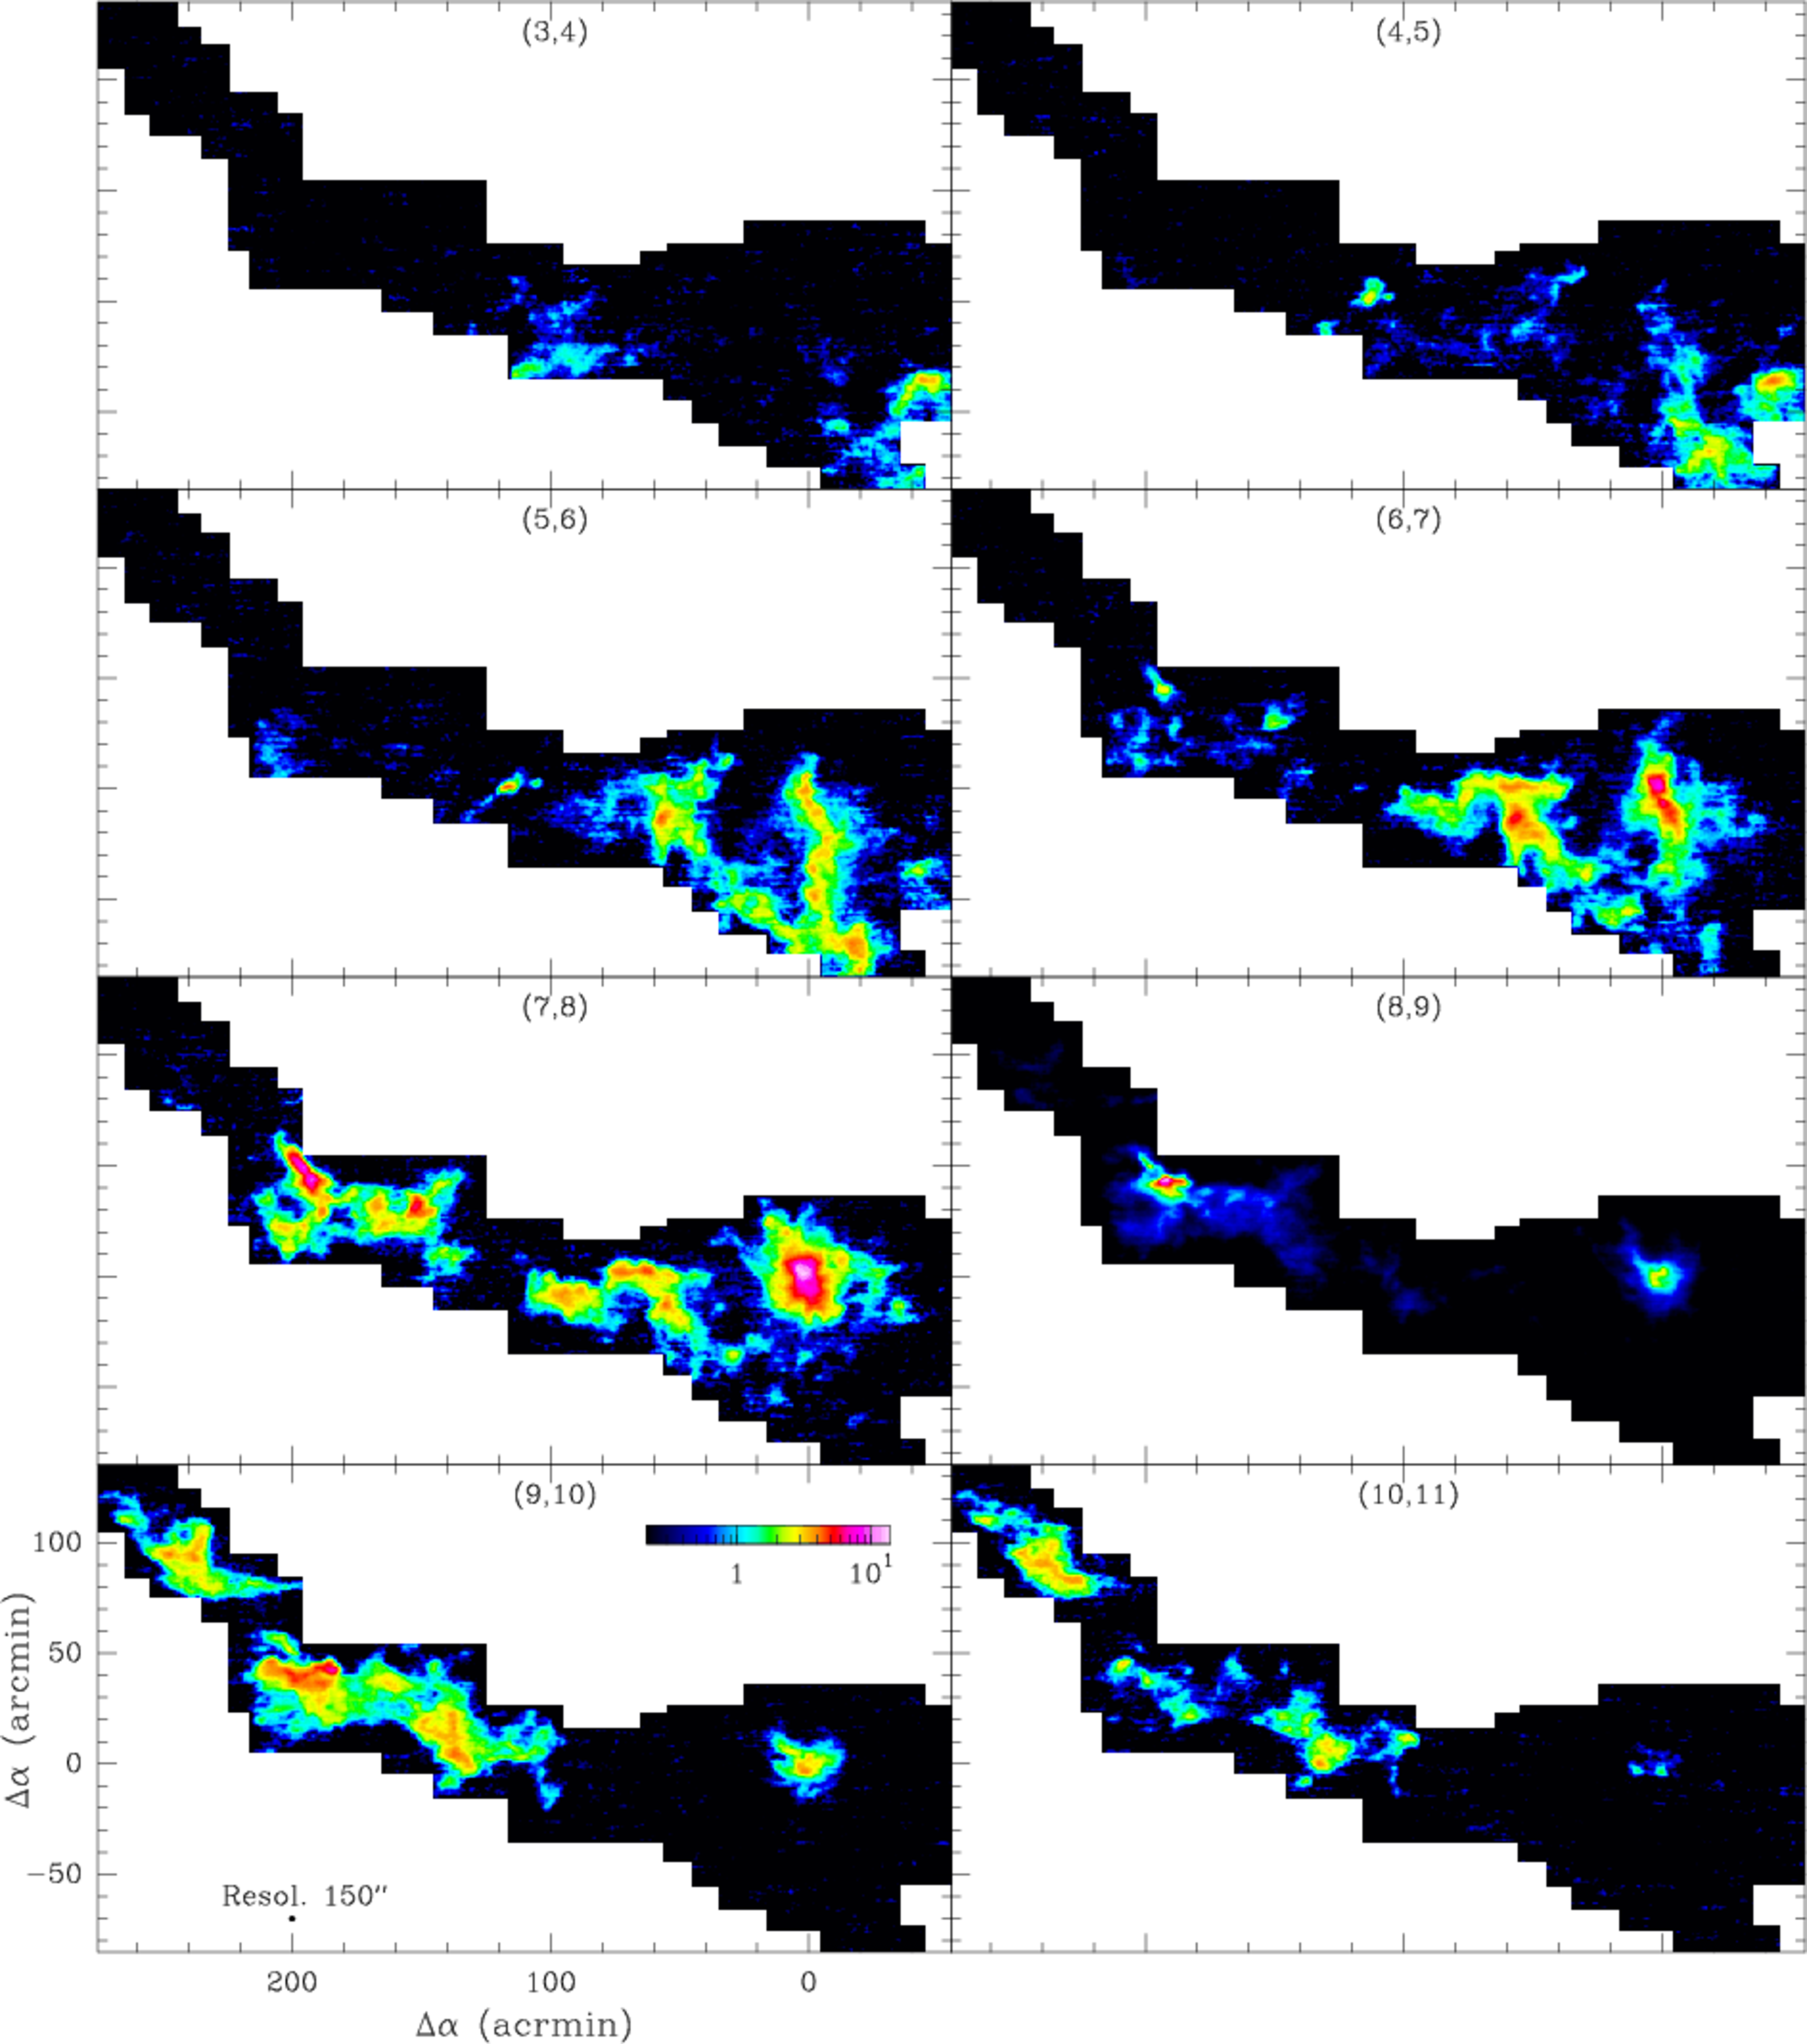
\includegraphics[width=\linewidth]{perseus_channel_sun06}
\caption[$^{13}$CO($2\rightarrow 1$) maps of Perseus]{
\label{fig:perseus_sun06}
Map of the Perseus cloud in $^{13}$CO($2\rightarrow 1$). The top panel shows the emission integrated over all velocities, while the bottom panel shows maps integrated over different velocity channels. In each sub-panel in the bottom, the numbers at the top indicate the velocity range (in km s$^{-1}$) of the emission shown. Credit: \citeauthor{sun06a}, A\&A, 451, 539, 2006, reproduced with
permission \copyright ESO.
}
\end{figure}

This complex structure on the sky is matched by a complex velocity structure. GMCs typically have velocity spreads that are much larger than the thermal sound speed of $\sim 0.2$ km s$^{-1}$ appropriate to 10 K gas. One can use different tracers to explore the distributions of gas at different densities in position-position-velocity space -- at every position one obtains a spectrum that can be translated into a velocity distribution along that line of sight. The data can be sliced into different velocities.

One can also get a sense of density and velocity structure by combining different molecular tracers. For example, the data set from COMPLETE (see Figure \ref{fig:complete_ridge06}) consists of three-dimensional cubes of $^{12}$CO and $^{13}$CO emission in position-position-velocity space, and from this one can draw isosurfaces. Generally the $^{12}$CO isosurfaces contain the $^{13}$CO ones, as expected since the $^{12}$CO traces less dense gas and the $^{13}$CO traces more dense gas. The density increases as one moves toward the cloud "center" in both position and velocity, but the morphology is not simple.   

\subsection{Cores}

As we zoom into yet smaller scales, the density rises to $10^5 - 10^7$ cm$^{-3}$ or more, while the mass decreases to a few $\msun$. These regions, called cores, tend to be strung out along filaments of lower density gas. Morphologically, cores tend to be closer to round than the lower-density material around them. These objects are thought to be the progenitors of single stars or star systems. Cores are distinguished not just by simple, roundish density structures, but by similarly simple velocity structures. Unlike in GMCs, where the velocity dispersion is highly supersonic, in cores it tends to be subsonic. This is indicated by a thermal broadening that is comparable to what one would expect from purely thermal motion.


